\chapter{Grundlagen von Datenbanken}
\bauer

	\section{Allgemeines zu Datenbanken}
	
	%Quelle: https://www.oracle.com/de/database/what-is-database/)
	\subsection{Definition}
	Eine Datenbank ist definiert als eine Sammlung von Informationen oder Daten welche im Normalfall auf einem elektronischen Medium wie einer Festplatte abgelegt werden. Der Zugriff auf die Daten erfolgt meist durch ein Verwaltungsprogramm. In den Grundzügen könnte die Daten auch simple Textdateien oder Papier sein welche per Hand befüllt und ausgewertet werden. Dies ist allerdings nicht die Norm. In der Industrie werden meist Datenbankverwaltungssystem benutzt welche von einem externen Anbieter zur Verfügung gestellt werden (Oracle, MongoDatabase, Microsoft SQL Server).
	
	%Quelle: https://www.mongodb.com/nosql-explained/nosql-vs-sql
	\subsection{Arten von Datenbank}
	In der Datenverarbeitung wird grundsätzlich zwischen zwei Arten von Datenbanken unterschieden auf der einen Seite gibt es SQL Datenbank und auf der anderen Seite NoSQL Datenbanken. Einer der größten Unterschiede dieser beiden Datenbank ist wie die Daten strukturiert und abgespeichert werden.
	
	%Quelle: https://de.wikipedia.org/wiki/SQL
	%Quelle: https://www.businessnewsdaily.com/5804-what-is-sql.html#:~:text=%2C%22%20Palic%20said.-,SQL%20history,Data%20Banks%2C%22%20in%201970.
	\subsubsection{SQL (Structured Query Language)}
	In einer SQL Datenbank werden die Daten durch eine klar definierte Struktur in Tabellen gespeichert und auf der Festplatte abgelegt. Die Structured Query Language früher bekannt als "SEQUEL" wurde in den 1970er von Raymond Boyce ond Donald Chaberlin welche damals bei IBM angestellt waren entwickelt. Zu diesem Zeitpunkt war SQL aber noch nicht für die Öffentlichkeit verfügbar, dies kam erst 1979 als eine Firma Namens "Relation Software" welche heutzutage unter dem Namen Oracle bekannt ist ihre Version der SQL Sprache als Oracle V2 auf den Markt gebracht haben.
	
	%Quelle: https://www.mongodb.com/nosql-explained/nosql-vs-sql
	\subsubsection{NoSQL (Not only Structured Query Language)}	
	In einer NoSQL Datenbank können Daten auf verschieden Arten organisiert und abgespeichert werden. Aber sämtliche dieser Methoden Unterscheiden sich vor allem auf eine Art von einer normalen SQL Datenbank. Dieser Unterschied liegt darin, dass die Datenbank nicht in konstanten Tabellen aufgebaut ist und dadurch eine höhere Flexibilität in den Daten ermöglicht. Ein Beispiel für eine solche Flexibilität ist die Speicherlösung welche die Firma "MongoDB" anbietet. In einer NoSQL Datenbank von diesem Anbieter werden die Daten in einzelnen JSON-Dateien geschrieben. Dies ermöglicht das jedes Element wenn benötigt eine eigene Struktur hat ohne das ein Schema vorgegeben oder angepasst werden muss. Eine weitere Sache welche in NoSQL Datenbank möglich ist die in SQL Datenbanken nicht so einfach realisierbar wäre ist die möglich in einem Datenobjekt ein Array von weiteren Datenobjekten zu speichern. Dies ermöglicht eine sehr hohe Flexibilität und war einer der Gründe warum wir uns bei unserem EMS Projekt auch für eine MongoDataBase entschieden haben.
	
	%Quelle: https://www.mongodb.com/nosql-explained/nosql-vs-sql
	\subsection{SQL vs NoSQL}
		Wie bereits vorher Beschrieben gibt es schon im Aufbau und in der Funktionsweise der Datenbank große Unterschiede in diesem Bereich werden die Vorteile und Nachteile der Datenbank Architekturen genauer beschrieben und gegenüber gestellt.
	
	%Quelle: https://becksche.de/Meldung/24-01-2014-sql-oder-nosql
	\subsubsection{SQL Vorteile}
		Um in einer SQL Datenbank etwas zu speichern muss immer ein Schema für die Datenbank vorher entwickelt und implementiert werden. Dieses Schema hat den Vorteil das direkt vom Anfang an bekannt ist welche Daten in der Datenbank gespeichert werden und wie die Datenbank aufgebaut wird. 
		Ein weiterer an dem Tabellen Aufbau ist die Einfachheit der Darstellung da die Daten ähnlich wie in einer Excel Tabelle angezeigt werden. Die Administration in einer SQL Datenbank ist ebenfalls einfacher da ins besondere für die weiter verbreitenden Datenbanksysteme wie Oracle oder Microsoft SQL Server viele Administrationstools existieren.
		
	\subsubsection{SQL Nachteile}
		Einer der Vorteile der SQL Datenbank ist gleichzeitig einer der Nachteile da ein Schema immer entworfen sein muss bevor die Datenbank befüllt werden kann, dies sorgt dafür, dass nachträgliche Änderungen der Struktur schwer zu bewerkstelligen sind da die alten Datensätze entweder aktualisiert oder teilweise mit dem Wert "Null" aufgefüllt werden müssen. Ein weiter Nachteil den viele Entwickler in einer SQL Datenbank sehen ist, dass aufteilen von Informationen über mehrere Tabellen. Wenn eine Datenmodellierung nach dem Lehrbuch durchgeführt wird muss die Datenbank am Ende der Modellierung in der dritten Normalform bestehen was in den meisten Fällen dafür sorgt, dass Daten auf mehreren Tabellen aufgeteilt sind um redundante Daten zu vermeiden. Diese Normalform verkompliziert allerdings oft die Abfragen da Joins benötigt werden um sämtliche Daten zu erhalten. Dazu kommt das diese Abfragen weniger Performant sind da mehrere Tabellen nach Informationen durchsucht werden müssen. 
		
	%Quelle: https://www.mongodb.com/nosql-explained/nosql-vs-sql
	\subsubsection{NoSQL Vorteile}
		Einer der größten Vorteile einer NoSQL Datenbank liegt in der Flexibilität des Datenmodels. Dieses Datenmodel hilft vor allem bei der Entwicklung einer Software wo die Anforderungen an die Datenbank nicht von Anfang an genau bekannt sind. Dies liegt daran, dass nicht von Anfang an ein Schema zum speichern der Daten benötigt wird da die einzelnen Objekte nicht in einer gewöhnlichen Tabelle gespeichert werden. Statt dessen werden die Daten in Objekte gespeichert welche nicht konsistent mit den anderen Objekten sein müssen. Dies bedeutet das es ein Objekt existieren kann welches Attribute besitzt die in den anderen Objekten nicht existieren. Ein weiterer Vorteil einer NoSQL Datenbank liegt darin, dass in einem Objekt ein Array von weiter Objekten gespeichert werden können dies wird in der Fachsprache als verschachteltes Array bezeichnet dies sorgt dafür das eine NoSQL fast nie Beziehungstabellen benötigt was Abfragen oft schneller macht da keine Joins benötigt werden. 
	
	%Quelle: https://www.mongodb.com/nosql-explained/nosql-vs-sql
	%Quelle: https://www.dnsstuff.com/de/nosql-datenbankvergleich#:~:text=Nachteile%20von%20NoSQL%2DDatenbanken&text=Erstens%20bieten%20NoSQL%2DDatenbanken%20nicht,wodurch%20ihre%20Systeme%20komplexer%20werden.
	\subsubsection{NoSQL Nachteile}
		Einer der Nachteile einer NoSQL Datenbank liegt darin das diese Datenbanken meist das ACID-Prinzip (Atomarität, Konsistenz, Isolation , Dauerhaftigkeit) nicht einhaltet was in manchen Fällen zu einer inkonsistent führen könnte. Allerdings gibt es die Möglichkeiten das die Entwickler ihren eigenen Code implementieren welcher das ACID-Prinzip einhält dies führt aber oft zu einem komplexeren Datenbanksystem. Ein weitere Nachteil der NoSQL Datenbank besteht darin, dass diese nicht mit der SQL-Sprache kompatible sind was die Lernkurve vor allem bei Entwicklern welche bis jetzt SQL verwendet haben erheblich anheben kann. Dazu kommt das Abfragen insbesondere wenn diese komplexer werden manchmal Performanceeinbußen entstehen können.
		
	\subsection{EMS Datenbank}
		In diesem Bereich wird auf den Datenbankaufbau in unseren Diplomarbeitsprojekt genauer eingegangen und die Gründe für unsere Entscheidungen sowohl den Aufbau betreffend als auch den Anbieter.
		
		%Quellen: https://www.mongodb.com/company#:~:text=MongoDB%20was%20founded%20in%202007,the%20shortcomings%20of%20existing%20databases.
		\subsubsection{Technologie}
			Für die EMS-Software hat sich unser Team für die MongoDB entschieden. Diese Datenbank baut auf JSON ähnliche Objekte auf welche Dokumente genannt werden. Jedes Dokumenten repräsentiert einen Datensatz, mehrere Dokumente sind in einer Kollektion zusammengefasst. Jedes Dokumenten hat beim erstellen einen Identifikator welche bei MongoDB mit '\_id' abgekürzt wird. Dieser Identifikator ist in der gesamten Datenbanken eindeutig, dass ist möglich da es sich um eine hexadezimal 12-Byte Zahl handelt. 
		
		\subsection{Anbieter}
			Unser Team hat sich für den Anbieter Atlas entschieden welcher Großkunden wie Adobe und Google. Die Firma wurde im Jahr 2007 von Dwight Merriman, Eliot Horowitz und Keyvin Ryan gegründet welche auch die Entwickler der Firma DoubleClick sind. Bei diesem Anbieter kann sich jeder eine gratis Datenbank erstellen welche über eine geteilte Cloud zur verfügbar gestellt wird. Für Geld kann die Datenbank auch direkt über Atlas auf einem dediziertem Server aufgesetzt werden welche zwischen 5€ und 1000€ pro Tag kosten können. Theoretisch könnte MongoDB auch auf seinem eigenen Rechner laufen lassen allerdings hat sich unser Team dagegen entschieden da die Administration von 4 nicht zentralen Datenbank während der Entwicklung ein zu großer Aufwand gewesen wäre
		
		\newpage		
		\subsubsection{Aufbau}
			Die Datenbank selbst ist in 2 Kollektionen aufgeteilt die Kollektion 'events' und die Kollektion 'users'. In der Kollektion 'events' werden alle Informationen zu einem spezifischen Event gespeichert und in der Kollektion 'users' werden die individuelle User der Applikation gespeichert sowohl Administratoren so wie die Promoter. Im nächsten Abschnitt werden die einzelnen Datenfelder der Dokumente benannt und der Verwendungszweck beschrieben.

			\subsubsection{Event Aufbau}			
				\begin{itemize}
					\item 'name' der Name des Events wird vor allem für die Anzeige benutzt
					\item 'creation\_date' das Datum gespeichert zudem ein Event erstellt wurde wird hauptsächlich in der Statistik verwendet
					\item 'expire\_date' das Datum gespeichert ab welchen Zeitpunkt es nicht mehr möglich ist Kartenverkäufe über die Applikation einzutragen wird benutzt um den User darin zu hindern Karten zu verkaufen nachdem die Zeit abgelaufen ist
					\item 'description' eine kurze Beschreibung des Events gespeichert um vor allem dem User die Identifikation einfacher zu machen
					\item 'early\_bird\_phase' eine Flagge gesetzt um zu speichern ob bei diesem Event eine Vorverkaufszeit aktiv
					\item 'early\_bird\_close' das Datum gespeichert wann einer der Administratoren die Vorverkaufszeit geschlossen hat
					\item 'cards' besteht aus einem Array aus Objekten
					\begin{itemize}
						\item card\_id' wird benutzt um Karten zu identifizieren (10 stellige zufällig generierte Nummer). 
						\item 'name' der Name der Karte
						\item "early\_bird" ist eine Flagge welche anzeigt das diese Karte nur als verkauft eingetragen werden kann während die Flagge 'early\_bird\_phase' aktiv ist
						\item 'amount' beschreibt die Anzahl an Karten die dieses Event hat
						\item 'price' ist der Preis der spezifischen Karte
					\end{itemize}
					\item 'packages' besteht aus einem Array aus Objekten
					\begin{itemize}
						\item 'package\_id' ist wie 'card\_id' ein Identifikator für die Packages (10 stellige zufällige Nummer)
						\item 'price' der Preis der spezifischen Karte
						\item 'name' der Name des Pakets
						\item 'price' der Preis des Pakets
						\item 'people' die Anzahl an Personen für die dieses Paket geplant wurde
						\item 'description' speichert die Details des Pakets
					\end{itemize}
					\item 'goodies' besteht aus einem Array aus Objekten
					\begin{itemize}
						\item 'goodie\_id' ist wie 'card\_id' und 'package\_id' ein Identifikator für die Belohnungen (10 stellige zufällige Nummer)
						\item 'name' der Name der Belohnungen
						\item 'points' die Punkte die benötigt werden um die Belohnung einzulösen
						\item 'description' die genauere Beschreibung der Belohnungen
					\end{itemize}				
				\end{itemize}
			
			\begin{figure}[h]
				\centering
				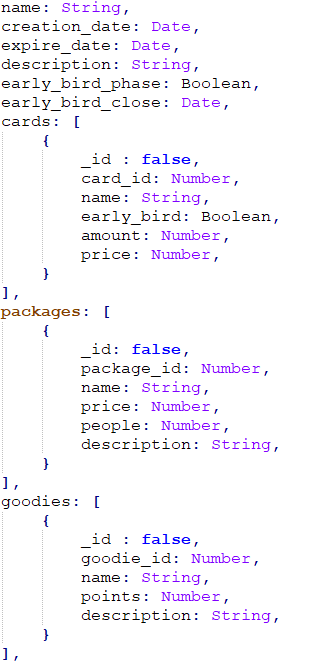
\includegraphics[width=\textwidth,height=\textwidth,keepaspectratio]{events_models.png}
				\caption{Event-Model}
			\end{figure}	
			
			\newpage		
				
			\subsubsection{User}
				\begin{itemize}
					\item 'firstname' der Vorname des User wird vor allem für die Anzeige benutzt
					\item 'lastname' der Nachname des User wird vor allem für die Anzeige benutzt
					\item 'username' der Username des User wird für das ein einloggen verwendet
					\item 'password' das Passwort des Users welches verschlüsselt abgespeichert wird
					\item 'email' die Email Adresse eines User wird vor allem zum Passwort zurücksetzen verwendet
					\item 'active' eine Flagge welche angibt ob ein User momentan aktiv seinen Kartenstand verändern kann
					\item 'admin' eine Flagge welche angibt ob dieser User ein Administrator ist
					\item 'description' eine kurze Beschreibung der Person die jeder User selbst verändern kann
					\item 'resetkey' der Schlüssel mit dem das Passwort zurückgesetzt wird wird nur für interne Überprüfungen benutzt
					\item 'request' eine Flagge welche angibt ob ein User eine Passwortzurücksetzung angefordert hat wird ebenfalls nur für interne Überprüfungen verwendet
					\item 'events' besteht aus einem Array von Objekten indem alle Events des Users gespeichert werden
					\begin{itemize}
						\item 'event\_id' ist die Identifikation des Events um welches es sich in diesem Objekt handelt (ObjektId des Events) in einer SQL Architektur würde man dies den Fremdschlüssel nennen
						\item 'active' eine Flagge welche angibt ob dieser User momentan bei diesem Event seinen Kartenstand verändern darf
						\item 'promotion\_start' das Datum an dem dieser User das Event das erste mal zugeteilt wurde wird für die Statistik verwendet
						\item 'points' der momentane Punktestand des User
						\item 'last\_changed' das Datum an dem der User das letzte mal seinen Kartenstand zu diesem Event aktualisiert hat
						\item 'mone\_submitted' der Betrag den der User bisher von den verkaufen Karten und Paket abgegeben hat
						\item 'cards' ist ein weiteres Array von Objekten
						\begin{itemize}
							\item 'card\_id' die Identifikationsnummer dieses Kartentyp
							\item 'amount' die Menge an Karten die ein User von diesem Kartentyp insgesamt bekommen hat
							\item 'sold' die Anzahl an Karten die der User von diesem Kartentyp verkauft hat
							\item 'submitted' die Anzahl an Karten die der User von diesem Kartentyp zurückgegeben hat
							\item 'available' die Anzahl an Karten von diesem Kartentyp welche der User noch im besitzt hat
						\end{itemize}
						\item 'goodies' ist ein weiteres Array von Objekten indem die eingelösten Goodies gespeichert werden
						\begin{itemize}
							\item 'goodie\_id' die Identifikationsnummer dieses Belohnungstyp
							\item 'date\_of\_redeem' das Datum an welchem diese Belohnung das letzte mal verändert wurde
							\item 'amount' Anzahl an Einlösung für diese Belohnung
						\end{itemize}
					\end{itemize}
				\end{itemize}

			\begin{figure}[h]
				\centering
				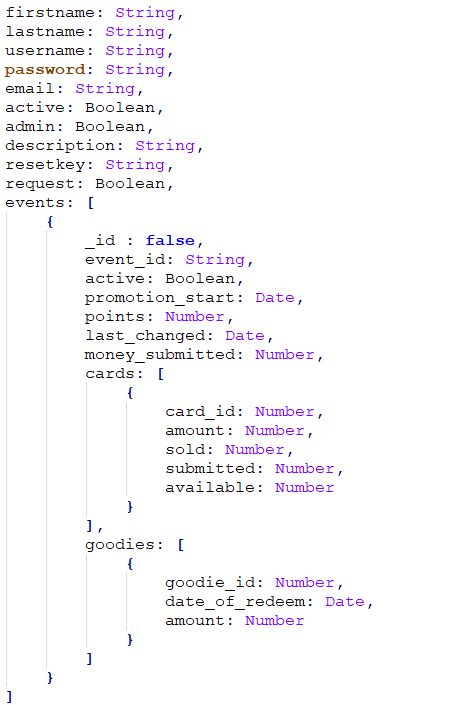
\includegraphics[width=\textwidth,height=\textwidth,keepaspectratio]{user_model.png}
				\caption{User-Model}
			\end{figure}
		
		\newpage
		\subsubsection{Entscheidungsgrundlagen}
			Einer der Gründe warum wir uns für die MongoDB entscheiden haben war, dass am Anfang niemand vorhersagen konnte wie genau unsere Datenbank aufgebaut sein wird. Während der Entwicklung gab es viele Informationen welche nachträglich in die Struktur eingefügt wurden dies hat uns dieser Anbieter sehr vereinfacht. Ein weiter Grund war, die Möglichkeit ein Array aus Objekten zu speichern was viel Abfragen und logistische Probleme gelöst hat ins besondere da wir in unserem Backend über die Schnittstelle "mongoose" auf die Datenbank zugreifen welche einiges ermöglicht was mit MonogDB alleine nicht realisierbar wäre wie zum Beispiel das Vorgeben einer Struktur welche aber veränderbar ist und auch ohne Update auf veralte Datensätze immer noch funktioniert. Diese Struktur ist hat uns auch ermöglicht das alle Mitglieder des Teams einen Überblick über die Datenbank bekommen und einfach Abfragen, Updates und Inserts schreiben konnten. Dazu kommt, dass durch die Möglichkeit der Arrays aus Objekten nur 2 Tabellen (Kollektion) benötigt werden während in einer normalen SQL Datenbank welche in dritter Normalform ist mindestens 12 Tabellen benötigt werden. Natürlich war uns die Performanz der Abfragen sehr wichtig was ein weiter Grund war warum wir uns für diese Technologie entschieden haben da die MongoDB eine sehr hohe Performanz hat selbst beim Abfragen von großen Dokumenten wie sie in unsere Datenbank gespeichert sind. Da die Objekte der MongoDB wie JSON Objekte aufgebaut sind hat das die Auswertung am Backend ebenfalls erleichtert.

\newpage